\documentclass{beamer}

\mode<presentation>{
\usetheme{Dresden}
\setbeamercovered{transparent}
\usecolortheme{lsc}
}

\mode<handout>{
  % tema simples para ser impresso
  \usepackage[bar]{beamerthemetree}
  % Colocando um fundo cinza quando for gerar transparências para serem impressas
  % mais de uma transparência por página
  \beamertemplatesolidbackgroundcolor{black!5}
}

\usepackage{amsmath}
\usepackage{amssymb}
\usepackage{amsthm}
\usepackage{ragged2e}
\usepackage[utf8]{inputenc}
\usepackage[brazil]{babel}
\usepackage{setspace}
\usepackage{amsmath}
\usepackage{amsfonts}
\usepackage{caption} 
\usepackage{amssymb}
\usepackage{graphicx}
\usepackage{booktabs}
\usepackage{color}	
\usepackage{xcolor}
\usepackage{scalefnt}
\usepackage{verbatim}
\usepackage{url}
\usepackage[alf]{abntex2cite}
\renewcommand{\tablename}{Table}
\renewcommand{\figurename}{Figure}



\beamertemplatetransparentcovereddynamic

\title{Transferências governamentais: uma análise de seu impacto no comportamento orçamentário dos municípios brasileiros}
\author[Pedro Jorge Holanda Alves]{Pedro Jorge Holanda Alves \\
Orientador: Dr. Jevuks Matheus Araújo}
  \institute[UFPB]{\\
  Universidade Federal da Paraíba \\ 
	\par
	Centro de Ciências Sociais Aplicadas \\
	\par
	Programa de Pós-Graduação em Economia \\}

% Se comentar a linha abaixo, irá aparecer a data quando foi compilada a apresentação  
\date{\today}

\pgfdeclareimage[height=1cm]{inf}{ufpb.png}

% pode-se colocar o LOGO assim
\logo{\pgfuseimage{inf}}



\AtBeginSection[]{
  \begin{frame}<beamer>
    \frametitle{Roteiro}
    \tableofcontents[currentsection,currentsubsection]
  \end{frame}
}

\begin{document}

\begin{frame}
\titlepage
\end{frame}

\begin{frame}
\frametitle{Roteiro}
\tableofcontents
\end{frame}

\section{Motivação}
\begin{frame}
	\frametitle{Motivação}
        \begin{itemize}
    \color{item}
    \item Teoria Normativa das Finanças Públicas
    \begin{itemize}
    \color{subitem}
        \item \citeonline{hayek1945use}
        \item \citeonline{samuelson1955diagrammatic}
        \item \citeonline{tiebout1956pure}
        \item \citeonline{oates1972fiscal}
            \end{itemize}
            \item Brasil
            \begin{itemize}
            \color{subitem}
                \item Constituição Federal (1988)
                \item Lei de Responsabilidade Fiscal (2000)
            \end{itemize}
                \item Objetivo principal
    \begin{itemize}
    \color{subitem}
    \justifying
        \item Verificar o comportamento orçamentário dos municípios em relação ao acrescimo de receita exógeno oriundo das transferências constitucionais entre 2013 e 2016 (gestão completa) usando as 3 primeiras faixas do FPM.
    \end{itemize}
    \end{itemize}
\end{frame}

\begin{frame}
	\frametitle{Motivação}
        \begin{itemize}
    \color{item}
    \item Objetivos específicos
    \begin{itemize}
        \justifying
        \item Replicar os resultados apenas para o ano eleitoral (2016)
        \item Replicar os resultados apenas para as duas primeiras faixas do FPM e para as três primeiras faixas separadas
    \end{itemize}
    \item Literatura empírica
    \begin{itemize}
        \item \citeonline{brollo2013political}
        \item \citeonline{litschig2013impact}
        \item \citeonline{lewis2017intergovernmental}  
        \begin{itemize}
        \color{subitem}
        \justifying
            \item Incentivo perverso é qualquer forma de incentivo que resulte em um resultado não desejado, não pretendido ou contrário aos interesses daqueles que originalmente promoveram o incentivo.
        \end{itemize}
        \item \citeonline{corbi2018regional}
        \item \citeonline{araujomatos2019} 
        \end{itemize}
    \end{itemize}
\end{frame}

\begin{frame}
	\frametitle{Informações Prévias}
        \begin{itemize}
    \color{item}
    \justifying
    \item Hipóteses
    \begin{itemize}
        \item Uso dos recursos adicionais na função administrativo ou com pessoal refletem em incentivos perversos; 
        \justifying
        \item O uso dos recursos adicionais podem gerar quedas na arrecadação própria (preguiça fiscal), que também é um tipo de incentivo perverso;
        \item Uso dos recursos adicionais na função saúde ou educação refletem em incentivos benéficos;
    \end{itemize}
    \item Regressão Descontínua
    \begin{itemize}
        \item Municípios próximos aos limiares tendem a ser parecidos;
        \item Não há indícios de manipulação nas Estimativas Populacionais;  
    \end{itemize}
    \item Resultados Obtidos
    \begin{itemize}
        \justifying
        \item Acrescimo de receita exógeno gera descontinuidade significativa apenas nos gastos na função administrativo via gastos com pessoal.
    \end{itemize}
    \end{itemize}
\end{frame}

\section{Metodologia}

\begin{frame} 
	\frametitle{Regressão Descontínua - Caso Sharp}
    \begin{itemize}
        \justifying
        \item É uma técnica estatística comumente usada para medir o efeito causal do recebimento de um tratamento binário;
        \item 3 Hipóteses:
        \begin{itemize}
            \item $Y(1),Y(0) \perp D$, X;
            \item Elementos abaixo do corte, sejam muito similares aos que estão um pouco acima deste;
            \item As esperanças condicionais são continuas em X.
        \end{itemize}
        \item Efeito Médio do Tratamento local
    \end{itemize}
    \begin{equation}
    \tau = lim_{x{\downarrow}c} E[Y_i|X_i=x] - lim_{x{\uparrow}c} E[Y_i|X_i=x]
\end{equation}
\begin{equation}
    Y = \alpha + D\tau + X\beta + \epsilon
\end{equation}
\end{frame}

\begin{frame} 
	\frametitle{Teste de McCrary (2008)}
    \begin{itemize}
    \item McCrary (2008) propõe a realização de um teste para identificar casos de manipulação na variável que gera a descontinuidade;
    \item O estimador obtido é uma extensão simples do estimador de densidade linear local em duas etapas (CHENG et al., 1997).
    \end{itemize}
    \begin{itemize}
            \item A primeira etapa se realiza para obter um histograma finamente em grade.
            \item O segundo passo suaviza o histograma usando regressão linear local separadamente, para ambos os lados do ponto de corte.
    \end{itemize}
\end{frame}

\begin{frame}
\begin{itemize}
    \item O teste serve como base para complementar as verificações de especificação existentes em regressão descontínua.
    \begin{itemize}
        \item Se as características específicas pré-determinadas são relevantes, este método deve ser informativo sobre qualquer classificação em torno da descontinuidade.
    \end{itemize}
    \item Tal teste é, de maneira natural e poderosa, para avaliar a plausibilidade das premissas identificadoras.
    \item O teste de densidade proposto complementa esses métodos, onde se espera que seja poderoso quando a manipulação for monotônica.
    \end{itemize}
    \begin{equation}
    Y_i = \alpha_i + \beta_iD_i = \overline{\alpha} + \overline{\beta}D_i + \epsilon_i
\end{equation}
\begin{itemize}
    \item Aceitar a hipótese de manipulação fazem com que os resultados sejam inconsistentes;
\end{itemize}
\end{frame}

\begin{frame} 
	\frametitle{Aplicação Empírica do RDD}
	\begin{itemize}
	    \justifying
	    \item Analisar os impactos das transferências
	    constitucionais do FPM no orçamento municipal;
	    \item Constitucionalmente é possível visualizar descontinuidade nas transferências do FPM pela população;
	    \item Possibilita um experimento quase natural que fornece instrumentos para estimar o efeito causal local do tratamento
	\end{itemize}
	
	\begin{equation}
    Y_{it} = \beta_0 + \tau_1 X_{it} + X(x) + \sum_{i=1}^{n} \theta_iX_{it} + \phi_{st} + \epsilon_{ir}
\end{equation}
	
	\vspace{-0.3cm}
\begin{align*}
 \tau &=
  \begin{cases}
   0        & \text{População} < C_i  \\
   1        & \text{caso contrário}
  \end{cases}
\end{align}
\end{frame}

\section{Breve Discurssão}

% Table generated by Excel2LaTeX from sheet 'fpm'
\begin{frame}
\begin{table} \tiny
  \caption{Coeficientes do FPM interior por faixa de habitantes.}
    \begin{tabular}{p{10.785em}lrr}
    \toprule
 \multicolumn{1}{|p{10.835em}|}{Faixa de habitantes} & \multicolumn{1}{c|}{\textbf{Coeficiente}} & \multicolumn{1}{p{10.085em}|}{Faixa de habitantes} & \multicolumn{1}{c|}{\textbf{Coeficiente}} \\
    \midrule
    \multicolumn{1}{|p{10.835em}|}{Até 10.188} & \multicolumn{1}{c|}{0.6} & \multicolumn{1}{|p{10.085em}|}{De 61.129 a 71.316} & \multicolumn{1}{c|}{2.4} \\
    \midrule
    \multicolumn{1}{|p{10.835em}|}{De 10.189 a 13.584} & \multicolumn{1}{c|}{0.8} & \multicolumn{1}{|p{10.085em}|}{De 71.317 a 81.504} & \multicolumn{1}{c|}{2.6} \\
    \midrule
    \multicolumn{1}{|p{10.835em}|}{De 13.585 a 16.980} & \multicolumn{1}{c|}{1.0} & \multicolumn{1}{|p{10.085em}|}{De 81.505 a 91.692} & \multicolumn{1}{c|}{2.8} \\
    \midrule
    \multicolumn{1}{|p{10.835em}|}{De 16.981 a 23.772} & \multicolumn{1}{c|}{1.2} & \multicolumn{1}{|p{10.085em}|}{De 91.693 a 101.880} & \multicolumn{1}{c|}{3.0} \\
    \midrule
    \multicolumn{1}{|p{10.835em}|}{De 23.773 a 30.564} & \multicolumn{1}{c|}{1.4} & \multicolumn{1}{|p{10.085em}|}{De 101.881 a 115.464} & \multicolumn{1}{c|}{3.2} \\
    \midrule
    \multicolumn{1}{|p{10.835em}|}{De 30.565 a 37.356} & \multicolumn{1}{c|}{1.6} & \multicolumn{1}{|p{10.085em}|}{De 115.465 a 129.048} & \multicolumn{1}{c|}{3.4} \\
    \midrule
    \multicolumn{1}{|p{10.835em}|}{De 37.357 a 44.148} & \multicolumn{1}{c|}{1.8} & \multicolumn{1}{|p{10.085em}|}{De 129.049 a 142.632} & \multicolumn{1}{c|}{3.6} \\
    \midrule
    \multicolumn{1}{|p{10.835em}|}{De 44.149 a 50.940} & \multicolumn{1}{c|}{2.0} & \multicolumn{1}{|p{10.085em}|}{De 142.633 a 156.216} & \multicolumn{1}{c|}{3.8} \\
    \midrule
    \multicolumn{1}{|p{10.835em}|}{De 50.941 a 61.128} & \multicolumn{1}{c|}{2.2} & \multicolumn{1}{|p{10.085em}|}{Acima de 156.216} & \multicolumn{1}{c|}{4.0} \\
    \midrule
    \multicolumn{4}{p{30.42em}}{Fonte: Decreto Lei nº 1.881/1981.} \\
    \end{tabular}%
  \label{tab02}%
\end{table}%    
\end{frame}

\begin{frame}
\begin{figure}[H]
    \caption{Faixas de população dos municípios e seus ganhos de FPM}
    \begin{center}
    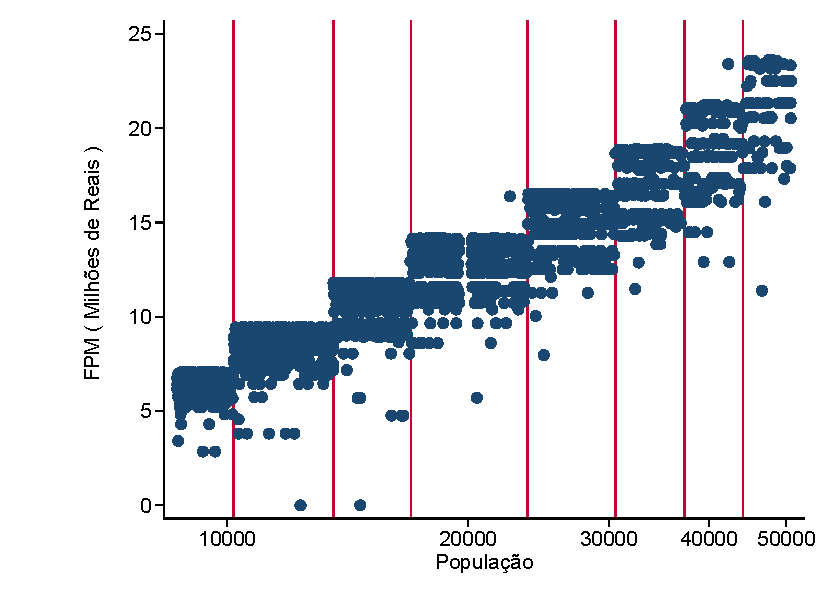
\includegraphics[scale=0.5]{Fpm.pdf}
    \end{center}
    \begin{flushleft}
    \vspace{-0.7cm}
     \caption*{Fonte: Elaboração própria, com base nos dados do IBGE. \\
    Nota: As linhas em vermelho representam os limiares populacionais especificados na tabela \ref{tab02}}
    \end{flushleft}
    \label{fig05}
\end{figure}    
\end{frame}

\begin{frame}
\begin{figure}[H]
    \centering
    \caption{Municípios ao longo do três primeiros tresholds (2016)}
    \vspace{-0.3cm}
    \includegraphics[scale=0.43]{threshold.png}
    \label{threshold}
\end{figure}
\end{frame}

\section{Testes}

\begin{frame}
	\frametitle{Teste McCray (2008)}
\begin{table}[H] \small
  \centering
  \caption{Resultado do teste de manipulação para população}
    \begin{tabular}{llllll}
    \toprule
    \multicolumn{1}{l|}{Faixas Populacionais} & \multicolumn{1}{c}{2\%} & \multicolumn{1}{c}{3\%} & \multicolumn{1}{c}{4\%} & \multicolumn{1}{c}{10\%} & \multicolumn{1}{c}{15\%} \\
    \midrule
    \multicolumn{1}{l|}{1º Faixa (10,188)} & \multicolumn{1}{r}{-1.4643} & \multicolumn{1}{r}{-1.4367} & \multicolumn{1}{r}{-0.9062} & \multicolumn{1}{r}{-1.071} & \multicolumn{1}{r}{-0.5797} \\
    \multicolumn{1}{l|}{Prob} & \multicolumn{1}{r}{0.1431} & \multicolumn{1}{r}{0.1508} & \multicolumn{1}{r}{0.3648} & \multicolumn{1}{r}{0.2842} & \multicolumn{1}{r}{0.5621} \\
    \midrule
    \multicolumn{1}{l|}{2º Faixa (13,584)} & \multicolumn{1}{r}{0.5903} & \multicolumn{1}{r}{0.5283} & \multicolumn{1}{r}{-0.2935} & \multicolumn{1}{r}{-0.3019} & \multicolumn{1}{r}{-0.7815} \\
    \multicolumn{1}{l|}{Prob} & \multicolumn{1}{r}{0.555} & \multicolumn{1}{r}{0.5973} & \multicolumn{1}{r}{0.7691} & \multicolumn{1}{r}{0.7628} & \multicolumn{1}{r}{0.4345} \\
    \midrule
    \multicolumn{1}{l|}{3º Faixa (16,980)} & \multicolumn{1}{r}{0.959} & \multicolumn{1}{r}{0.6227} & \multicolumn{1}{r}{-0.3091} & \multicolumn{1}{r}{-0.1085} & \multicolumn{1}{r}{-0.3504} \\
    \multicolumn{1}{l|}{Prob} & \multicolumn{1}{r}{0.3375} & \multicolumn{1}{r}{0.5335} & \multicolumn{1}{r}{0.7573} & \multicolumn{1}{r}{0.9136} & \multicolumn{1}{r}{0.726} \\
    \midrule
    \multicolumn{6}{l}{Fonte: Elaboração própria} \\
    \end{tabular}%
  \label{manipulacao}%
\end{table}%
\end{frame}

\begin{frame}
	\frametitle{Descontinuidade nas transferências}
\begin{table}[H]%
    \centering
    \caption{Descontinuidade nas receitas}%
    \includegraphics[scale=0.5]{Graph1.pdf} %
    \begin{flushleft}
        \vspace{-0.4cm}

    Fonte: Elaboração própria com base nos dados do IBGE e STN
    \end{flushleft}
    \label{graph1}%
\end{table}
\end{frame}

\begin{frame}
	\frametitle{Teste de Placebo}
\begin{table}[H]%
    \centering
    \caption{Teste de Placebo (Pop = 5000 e Pop = 20000)}%
    \includegraphics[scale=0.8]{Teste_placebo.pdf} %
    \begin{flushleft}
        \vspace{-0.4cm}

    Fonte: Elaboração própria com base nos dados do IBGE e STN.
    \end{flushleft}
    \label{graph1}%
\end{table}
\end{frame}

\begin{frame}
	\frametitle{Teste de descontinuidade nas covariadas}
\begin{table}[H] \tiny
  \centering
  \caption{Teste de descontinuidade para as covariadas}
  \begin{tabular}{l*{4}{c}}
  \hline
  \textit{Bandscale} &\multicolumn{1}{c}{4\%}&\multicolumn{1}{c}{5\%}&\multicolumn{1}{c}{10\%}&\multicolumn{1}{c}{15\%}\\
  \hline
  \multicolumn{4}{l}{\textbf{Distância}}\\
   & -29.017 & -30.150 & -18.666 & -7.257 \\
 & (21.408) & (18.877) & (13.132) & (11.453) \\
Observations & 1,687 & 2,117 & 4,478 & 6,130 \\
  \hline
    \multicolumn{4}{l}{\textbf{Empresas}}\\
   & -25.364 & -15.826 & -32.598* & -31.914** \\
 & (28.409) & (25.586) & (17.884) & (15.994) \\
Observations & 1,687 & 2,117 & 4,478 & 6,130 \\
  \hline
    \multicolumn{4}{l}{\textbf{Empregados}}\\
   & -251.141 & -111.690 & -182.863* & -177.522** \\
 & (160.400) & (140.284) & (97.228) & (83.912) \\
Observations & 1,687 & 2,117 & 4,478 & 6,130 \\
  \hline
  \multicolumn{4}{l}{\textbf{PIB}}\\
   & -324.616 & -222.925 & -85.410 & -161.430 \\
 & (354.297) & (313.694) & (271.761) & (267.278) \\
Observations & 1,687 & 2,117 & 4,478 & 6,130 \\
  \hline
  \multicolumn{4}{l}{\textbf{Possibilidade de Reeleição}}\\
   & 0.043 & 0.056 & 0.062* & 0.017 \\
 & (0.057) & (0.051) & (0.036) & (0.032) \\
Observations & 1,687 & 2,117 & 4,478 & 6,130 \\
  \hline
  \multicolumn{5}{l}{Elaboração própria} 
\end{tabular}
\end{table}
\end{frame}

\section{Resultados}

\begin{frame}
	\frametitle{Descontinuidade na Receita e Despesa}
\begin{table}[H]%
    \centering
    \caption{Descontinuidade da despesa e receita}%
    \includegraphics[scale=0.5]{Graph2.pdf} %
    \begin{flushleft}
        \vspace{-0.4cm}

    Fonte: Elaboração própria com base nos dados do IBGE e STN
    \end{flushleft}
    \label{receita}%
\end{table}
\end{frame}

\begin{frame}
	\frametitle{Descontinuidade no tipo de despesa}
\begin{figure}[H]
    \centering
    \caption{Descontinuidade dos gastos com pessoal e capital}
    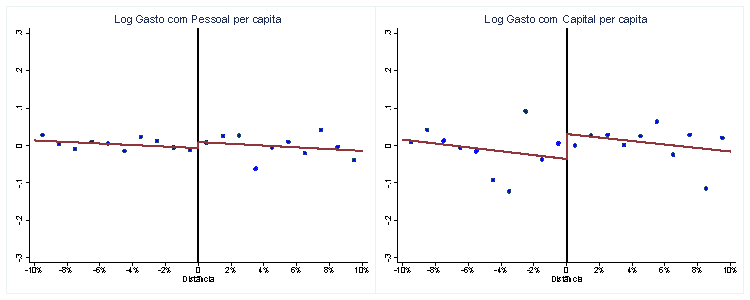
\includegraphics[scale=0.8]{Graph6.pdf}
    \begin{flushleft}
    \vspace{-0.4cm}
    Fonte: Elaboração própria com base nos dados do IBGE e STN
    \end{flushleft}
    \label{rdd_funcao}%
\end{figure}
\end{frame}

\begin{frame}
	\frametitle{Descontinuidade no tipo de despesa}
 \begin{figure}[H]%
    \centering
    \caption{Descontinuidade dos gastos na função Educação, Saúde, Administrativo e Legislativo}%
    \includegraphics[scale=0.5]{Graph3.pdf} %
    \begin{flushleft}
        \vspace{-0.4cm}
    Fonte: Elaboração própria com base nos dados do IBGE e STN
    \end{flushleft}
    \label{funcao1}%
\end{figure}
\end{frame}

\begin{frame}
	\frametitle{Descontinuidade no tipo de despesa}
\begin{figure}[H]%
    \centering
    \caption{Descontinuidade dos gastos na função Urbanismo, Cultura, Desportivo e Lazer e Transporte}%
    \includegraphics[scale=0.5]{Graph4.pdf} %
    \begin{flushleft}
        \vspace{-0.4cm}
    Fonte: Elaboração própria com base nos dados do IBGE e STN
    \end{flushleft}
    \label{funcao2}%
\end{figure}
\end{frame}

\begin{frame}
	\frametitle{Descontinuidade no tipo de função}
 \begin{figure}[H]%
    \centering
    \caption{Descontinuidade dos gastos na função Encargos Especiais e Previdência}%
    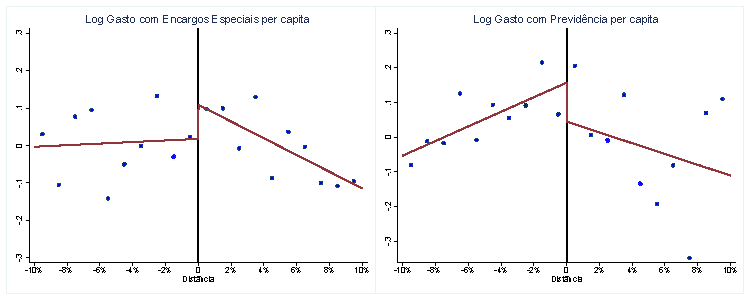
\includegraphics[scale=0.8]{Graph5.pdf} %
    \begin{flushleft}
        \vspace{-0.4cm}

    Fonte: Elaboração própria com base nos dados do IBGE e STN
    \end{flushleft}
    \label{funcao3}%
\end{figure}
\end{frame}

\section{Considerações Finais}

\begin{frame}
\begin{itemize}
    \item Acréscimos de receita exógeno geram aumentos de gastos com pessoal. Este resultado torna significativo apenas com a inclusão das co-variadas.
    \item Forte significância estatística dos gastos com administrativo. Os aumentos dos gastos com pessoal situam como os gastos com administrativo estão sendo realizados.
    \item Por outro lado, os demais gastos, como despesa com educação, saúde, segurança pública e transporte não apresentaram sofrer nenhum impacto das transferências adicionais do FPM.
\end{itemize}
\end{frame}	

\begin{frame}
    \frametitle{Considerações Finais}
    \begin{itemize}
    \item O gasto defasado espacialmente mostra-se relevante para o impacto do gasto local.
    \item Em 2016 (ano eleitoral) os resultados se repetem e apresentam coeficientes mais intensos quando são comparados com os resultados do painel (gestão completa).
    \item Apesar de não ser muito significativo, a descontinuidade do indicador de Autonomia do Índice Firjan de Gestão Fiscal da indícios da perda de eficiência da descontinuidade positiva dos gastos na administração pública da prefeitura na autonomia municipal.
\end{itemize}
\end{frame}

\begin{frame}{Referências Bibliográficas}

    \tiny{\bibliography{referencias}}
\end{frame}

\begin{frame}{Repositório no Github}
\begin{center}
    \item github.com/PedroJorge7/Dissertation
\end{center}
\end{frame}

\begin{frame}
\begin{center}
    Obrigado Pela Atenção!
\end{center}
\end{frame}

\end{document}